\section{Evaluación empírica}

Para evaluar el rendimeinto, se ha usado el \textit{script} de Python \href{run:./src/test.py}{\texttt{src/test.py}}.\\
Se ha ejecutado cada función en todo el rango de valores posibles que permite el sistema, desde números un dígito, hasta lo máximo posible, en este caso números de 20 digitos. Para obtener dicho número máximo, se emplean la variables \texttt{primeslib.MAX\_UINT} y \texttt{gcdlib.MAX\_INT} que retonan el mayor número posible de computar para cada librería.\\
\\
Para cada longitud de numeros se calculan un total de 400 numeros aleatorios y se aplica la función a cada uno de ellos para determinar si son primos. Así se obtiene la media de tiempo de ejecución para dicha longitud de número, buscando obtener resultados lo más fiables posible, evitando así que los casos extremos distorsionen dichos resultados.\\

Una vez obtenidos los resultado indicados previamente, se guardan en formato CSV en la carpeta \texttt{data/} y se representan gráficamente mediante la librería \href{https://matplotlib.org/}{matplotlib}.

\subsection{Test de primalidad}
Se comprueba como el tiempo de ejecución se mantiene estable con pequeñas variaciones para números de hasta 15 digitos, de ahí en adelante se aprecia que cada aumento de tamaño de número se traduce en un aumento cada vez más significativo en el tiempo de ejecución.\\
\\
Pese a que el grafico muestre una distribución de resultados logarítmica, esto se debe a que la escala muestra en el eje x el numero de digitos de los números, por lo tanto la escala no avanza de manera lineal ya que por cada digito que aumenta, la cantidad de números aumenta en mayor medida que para el número de digtos previo. Es por ello, que pese a que se muestre una distribución logarítmica, si la escala empleada para mostrar el gráfico fuese lineal se mostraría el grafico de manera lineal. A continuación se incluye dicho grafico:

\begin{figure}[H]
	\makebox[\textwidth][c]{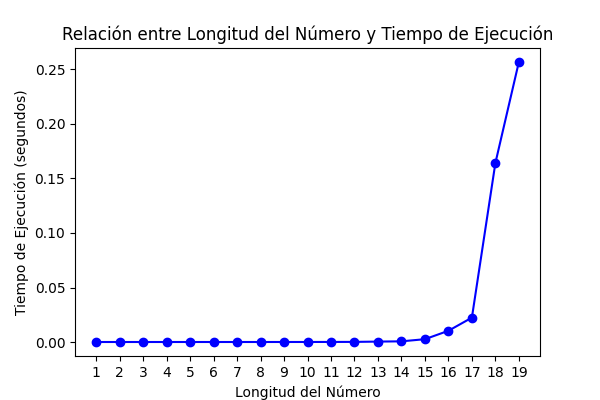
\includegraphics[width=15cm]{img/scatter_plot_primes.png}}
\end{figure}

Adicionalmente al grafico previo, se incluye el gráfico recogiendo los tiempos de ejecución únicamente para los números primos, donde se observa que la tendencia cambia mostrando un incremento de tiempo de ejecución más pronunciado desde el comienzo.
\begin{figure}[H]
	\makebox[\textwidth][c]{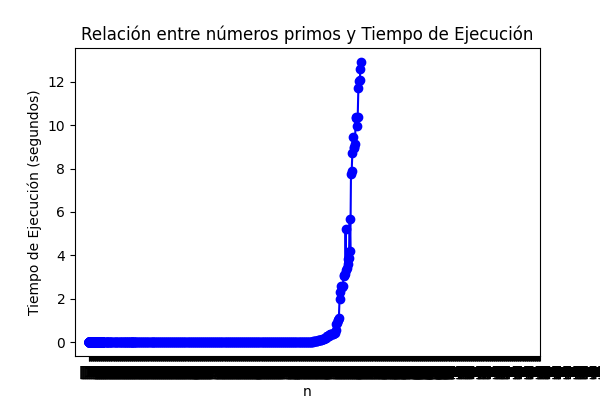
\includegraphics[width=15cm]{img/scatter_plot_primes_only_primes.png}}
\end{figure}

\subsection{Cálculo de Máximo Común Divisor}

\subsubsection{Descomposición en factores primos}
Debido al tiempo de ejecución, para esta prueba redujimos el número de iteraciones a 5 y el máximo de dígitos a 11.
\begin{figure}[H]
	\makebox[\textwidth][c]{\includegraphics[width=15cm]{img/scatter_plot_gcd_factorize.png}}
\end{figure}


\subsubsection{Método de Euclides}
\begin{figure}[H]
	\makebox[\textwidth][c]{\includegraphics[width=15cm]{img/scatter_plot_gcd_euclid.png}}
\end{figure}